\section{Introduction}


\subsection{Overview}

Edges in real-world networks are often directed, such as links on the world wide web, ``follows'' on Twitter, financial transactions or disease transmission in a social network. When analysing networks, the first quantity that is often considered is the distribution of the degrees of nodes in the network.  In this paper we will consider sampling an i.i.d.\ sequence of in- and out-degrees, conditional on the total in-degree being equal to the total out-degree. We will then sample a uniform directed graph (digraph) with the given degree sequence. Results on such graphs are a useful benchmark, exposing additional underlying structure of a real-world network compared to a uniformly random graph with its degree sequence.

When considering such models, previous work by \citet{cooperSizeLargestStrongly2004} (which we will discuss in more detail in Section \ref{sec.previouswork}) shows that there exists a phase transition in the strong directed connectivity of the graph. Two vertices are part of the same \emph{strongly connected component} (SCC) if and only if there exists a directed cycle that contains both of them. Above some threshold, there will exist a unique giant SCC that occupies a positive proportion of the vertices whereas, below the threshold no SCC will occupy a positive proportion of the vertices. In Figure \ref{fig.SCCs}, a directed graph and its strongly connected components are depicted. In this paper we will prove the first detailed results about the critical case - specifically, that there exists a sequence of random weighted directed multigraphs that can be understood as the scaling limit of the SCCs when viewed in decreasing order of size.

\subsection{Directed graphs}

\begin{figure}
    \centering
    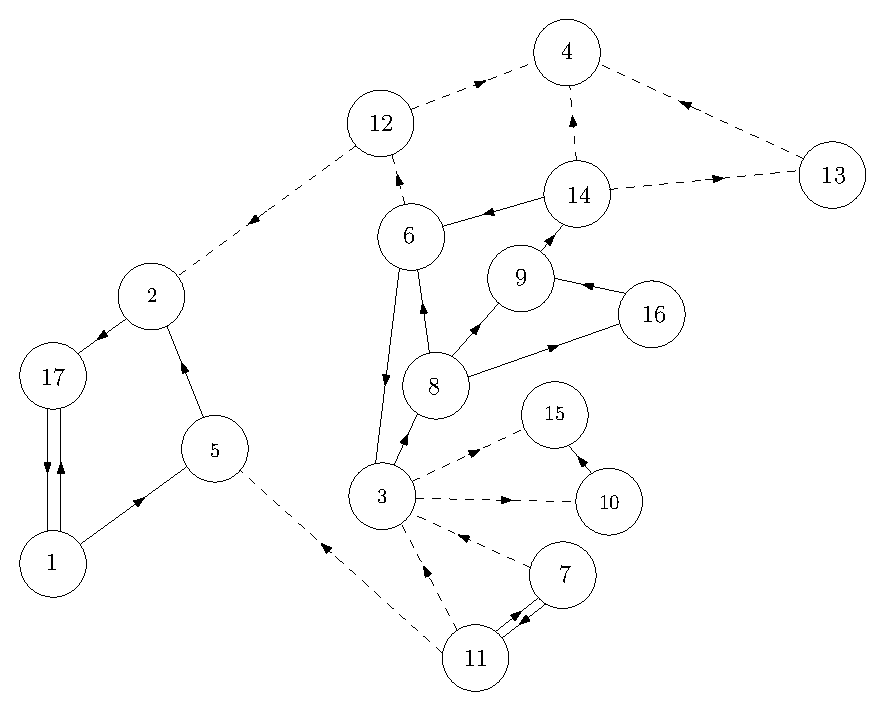
\includegraphics[scale=0.6]{Content/Pictures/Fig1.eps}
    \caption{A directed graph on [17]. The strongly connected components have vertex sets $\{1,2,5,17\}$, $\{3,6,8,9,14,16\}$, $\{7,11\}$, $\{4\}$, $\{10\}$, $\{12\}$, $\{13\}$, and $\{15\}$. Edges that are not part of an SCC are depicted as dashed arrows. Taken from \cite{goldschmidtScalingLimitCritical2021} with permission of the authors.}
    \label{fig.SCCs}
\end{figure}

There are two notions of connectivity when working with a directed graph: weak and strong connectivity. We will be working with the strong notation. We say a vertex $v$ leads to a vertex $w$, written $v \rightarrow w$, if there exists a directed path from $v$ to $w$ in the graph. We say $v$ is \emph{strongly connected to $w$}, written $v \leftrightarrow w$, if $v$ leads to $w$ and $w$ leads to $v$. By convention, $v$ leads to itself. A graph is \emph{strongly connected} if all pairs of vertices in the graph are strongly connected. The relation $v \leftrightarrow w$ is an equivalence relation; the digraphs induced by the equivalence classes of $\leftrightarrow$ are referred to as the \emph{strongly connected components} (SCCs). For each vertex $v$ in a directed graph $\vec{G}$, we will use the notation $d^-(v)$ for the in-degree of $v$ and $d^+(v)$ for the out-degree of $v$. Moreover, a directed edge $(v,w)$ has \emph{tail} $v$ and \emph{head} $w$ (see Figure \ref{fig.tailhead}).
\begin{figure}
    \centering
    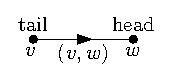
\includegraphics{Content/Pictures/Fig2.eps}
    \caption{An edge $(v,w)$ will be depicted as an arrow from $v$ to $w$.}\label{fig.tailhead}
\end{figure}


\subsection{Description of the model}

\label{subsec:model-description}

First consider a deterministic degree sequence $\vd_1, \ldots, \vd_n$ where $\vd_i = (d_i^-, d_i^+)\in \N \times \N$ for $i = 1, \ldots, n$. We say a directed graph with vertex set $[n]$, where $[n] = \{1,\dots,n\}$, has degree sequence $\vd_1, \ldots, \vd_n$ if $(d^-(i), d^+(i)) = (d_i^-, d_i^+)$ for $i = 1, \ldots, n$.

In order to sample a uniformly random graph with a given degree sequence, we first consider the \emph{directed configuration model} introduced by \citet{cooperSizeLargestStrongly2004}. Take $n$ vertices $v_1, \ldots, v_n$ such that $v_i$ has $d^-_i$ in-half-edges and $d^+_i$ out-half-edges. Then construct a multigraph by choosing a uniformly random pairing of the in-half-edges with the out-half-edges. \citet[Sec.\ 2.1]{cooperSizeLargestStrongly2004} proved that if we condition on the resulting multigraph being simple, we obtain a uniformly chosen random digraph with the given degree sequence.

In this paper we will consider the case where the degree sequence  consists of $n$ i.i.d.\ random variables conditioned on the total in-degree being equal to the total out-degree. Let $\nu$ be a distribution on $\N \times \N$, and let $\vD_1, \ldots, \vD_n$ be a sequence of i.i.d.\ random variables with distribution $\nu$. We condition on the event
\begin{equation*}
    \left\{ \textstyle \sum_{i=1}^n D_i^- = \sum_{i=1}^n D_i^+ \right\},
\end{equation*}
observing that this is an asymptotically singular event as $n\to\infty$. Let $\vec{G}_n(\nu)$ be a digraph chosen uniformly at random from all digraphs with degree sequence $\vD_1, \ldots, \vD_n$. We are interested in the limit under rescaling of the SCCs of $\vec{G}_n(\nu)$ as $n\to \infty$.

Suppose $(D^-, D^+)$ has law $\nu$. We will require the following assumptions to hold:
\begin{enumerate}
    % \item $\E[(D^-) + D^+)^3] < \infty$,
    \item $\E[(D^-)^i(D^+)^j]< \infty$ for $1 \leq i+j\leq 3$, $(i, j) = (1, 3)$ and $(i, j) = (3, 1)$.
    \item $\E[D^-] = \E[D^+]$.
    \item $D^- - D^+$ is strongly aperiodic. This means that for all $p > 1$, there does not exist $k \in \Z$ such that 
    \begin{equation*}
        \P(D^- - D^+ \in k + p\Z) = 1.
    \end{equation*}
    \item $\E[D^-D^+] = \E[D^-]$ or $\E[D^- D^+] = \E[D^+]$, where both statements are equivalent supposing the second condition holds.
\end{enumerate}

The first condition is required to ensure that the steps of a random walk used in the proof have finite variance, so that the random walk will convergence under rescaling to a Brownian motion. It also ensures similar regularity of other random variables that we use to encode the directed graph. (We discuss relaxing the moment conditions in \Cref{subsec.openproblems}.)

The second and third conditions make sure the event $\{\sum_{i=1}^n D^-_i = \sum_{i=1}^n D^+_i\}$ is well-behaved. The second condition ensures that it is not a large deviation event. Using a result from \citet[Page 42, P1]{spitzerPrinciplesRandomWalk1964}, the third condition ensures that the event has positive probability for all sufficiently large $n \geq 1$. This condition can be relaxed to assuming that $D^- - D^+$ is non-constant by taking limits for $n \in p \N$ rather than $n \in \N$ where $p$ is the periodicity of $D^- - D^+$. However, for simplicity of presentation, we will keep it as an assumption.

The fourth assumption is the criticality condition. To understand how this arises, consider the directed configuration model and let $(V_n, W_n)$ be a uniformly chosen edge. For now, ignore the conditioning on the total in- and out-degrees being equal. We consider the distribution of the in- and out-degree of $W_n$. Because the degree sequence is an i.i.d.\ sequence, $W_n$ is equally likely to be any vertex $i$. Thus for any $\vk = (k^-, k^+)$,
\begin{align*}
    \P(d^-(W_n) = k^-, d^+(W_n) = k^+)
    &= n \P(W_n = 1, \vD_1 = \vk) \\
    &= n \E[\P(W_n = 1 \mid \vD_1 = \vk, \vD_2, \ldots, \vD_n)] \P(\vD_1 = \vk)
\end{align*}
Conditionally on the degree sequence, we have that $W_n = i$ with probability proportional to $D^-_i$ since we used an uniform pairing of the in- and out-half-edges. Therefore
\begin{align*}
    \P(W_n = 1 \mid \vD_1 = \vk, \vD_2, \ldots, \vD_n)
    &= \frac{k^-}{k^- + \sum_{i=2}^n D_i^-}.
\end{align*}
Thus
\begin{equation*}
    \P(d^-(W_n) = k^-, d^+(W_n) = k^+) = \E\left[ 
        \frac{k^-}{\frac{1}{n}\left( k^- + \sum_{i=2}^n D_i^- \right)}
    \right]
    \P \left[ D^- = k^-, D^+ = k^+ \right].
\end{equation*}
Using the law of large numbers, the above will converge to
\begin{equation*}
    \frac{k^-}{\E[D^-]} \P\left[ D^- = k^-, D^+ = k^+ \right].
\end{equation*}
Let $(Z^-, Z^+)$ be such that $P(Z^- = k^-, Z^+ = k^+)$ is given by the above expression. We say $(Z^-, Z^+)$ has the law of the \emph{degree distribution size-biased by in-degree}. For large $n$, any other fixed out-edge of $W_n$ is then also distributed approximately like a uniformly chosen edge (here we are ignoring the fact that we have already sampled an edge) since we chose the in- and out-edge pairing uniformly at random. Therefore the out-degree of the head will have approximately the same distribution as $Z^+$. Thus if we were to look at the graph of all vertices leading from $W_n$, it would look approximately like a Bienaymé tree\footnote{For $\mu$ a probability distribution on $\N$, a Bienaymé tree with offspring distribution $\mu$ is the family tree of a branching process with offspring distribution $\mu$. Bienaymé trees are often referred to as Galton--Watson trees, but we decide to follow the name change suggested by \citet{addario-berryUniversalHeightWidth2021}.} with offspring distribution $Z^+$. It is well known that such trees exhibit critical behaviour in whether or not the tree is finite at $\E[Z^+] = 1$. This is equivalent to assuming $\E[D^-D^+] = E[D^-]$.

\citet{cooperSizeLargestStrongly2004} studied this phase transition for a deterministic degree sequence $\vd_1, \ldots, \vd_n$. They defined the parameter
\begin{equation*}
    d = \frac{\sum_{i=1}^n d_i^+ d_i^-}{\sum_{i=1}^n d_i^-}
\end{equation*}
which is a counterpart of $\E[Z^-]$ for deterministic degree sequences. They then showed that, under additional assumptions, there exists a phase transition for the existence of a giant SCC depending on whether $d$ is strictly greater than or less than 1. Our work in this paper shows our corresponding condition, $\E[Z^-] = 1$, is also the correct criticality condition to take for i.i.d.\ random degree sequences.

We define the following parameters that will determine the behaviour of the SCCs in the limit.
\begin{enumerate}
    \item $\mu:=\E[D^-]=\E[D^+]=\E[D^-D^+]$
    \item $\nu_-:= \E[Z^-] - 1 = \frac{\E[(D^-)^2]-\mu}{\mu}$ 
    \item $\sigma_-^2 := \var(Z^-) = \frac{\mu\E[(D^-)^3]-\E[(D^-)^2]^2}{\mu^2}$ 
    \item $\sigma_+^2 := \var(Z^+) = \frac{\E[D^-(D^+)^2]-\mu}{\mu}$ 
    \item $\sigma_{-+} := \cov(Z^-, Z^+) = \frac{\E[(D^-)^2D^+]-\E[(D^-)^2]}{\mu}$ 
\end{enumerate}
% \begin{remark}
% Conditions \ref{cond.beta} and \ref{cond.gamma} ensure that the Central Limit Theorem applies to the fluctuations of the first explored in-degrees around their mean. Condition \ref{cond.critical} ensures that the branching process corresponding to the depth-first exploration (i.e. the exploration of the out-components) is critical. Condition \ref{cond.rho} ensures that this branching process has Brownian scaling. Condition \ref{cond.tau} ensures that the covariance of the in- and out-degrees that are discovered first is finite. Condition \ref{cond.iota} ensures that the strongly connected components are $3$-regular. 
% \end{remark}
\subsection{Metric directed multigraphs and kernels}\label{subsec.mdmkernels}

\begin{figure}[htbp]
    \centering

    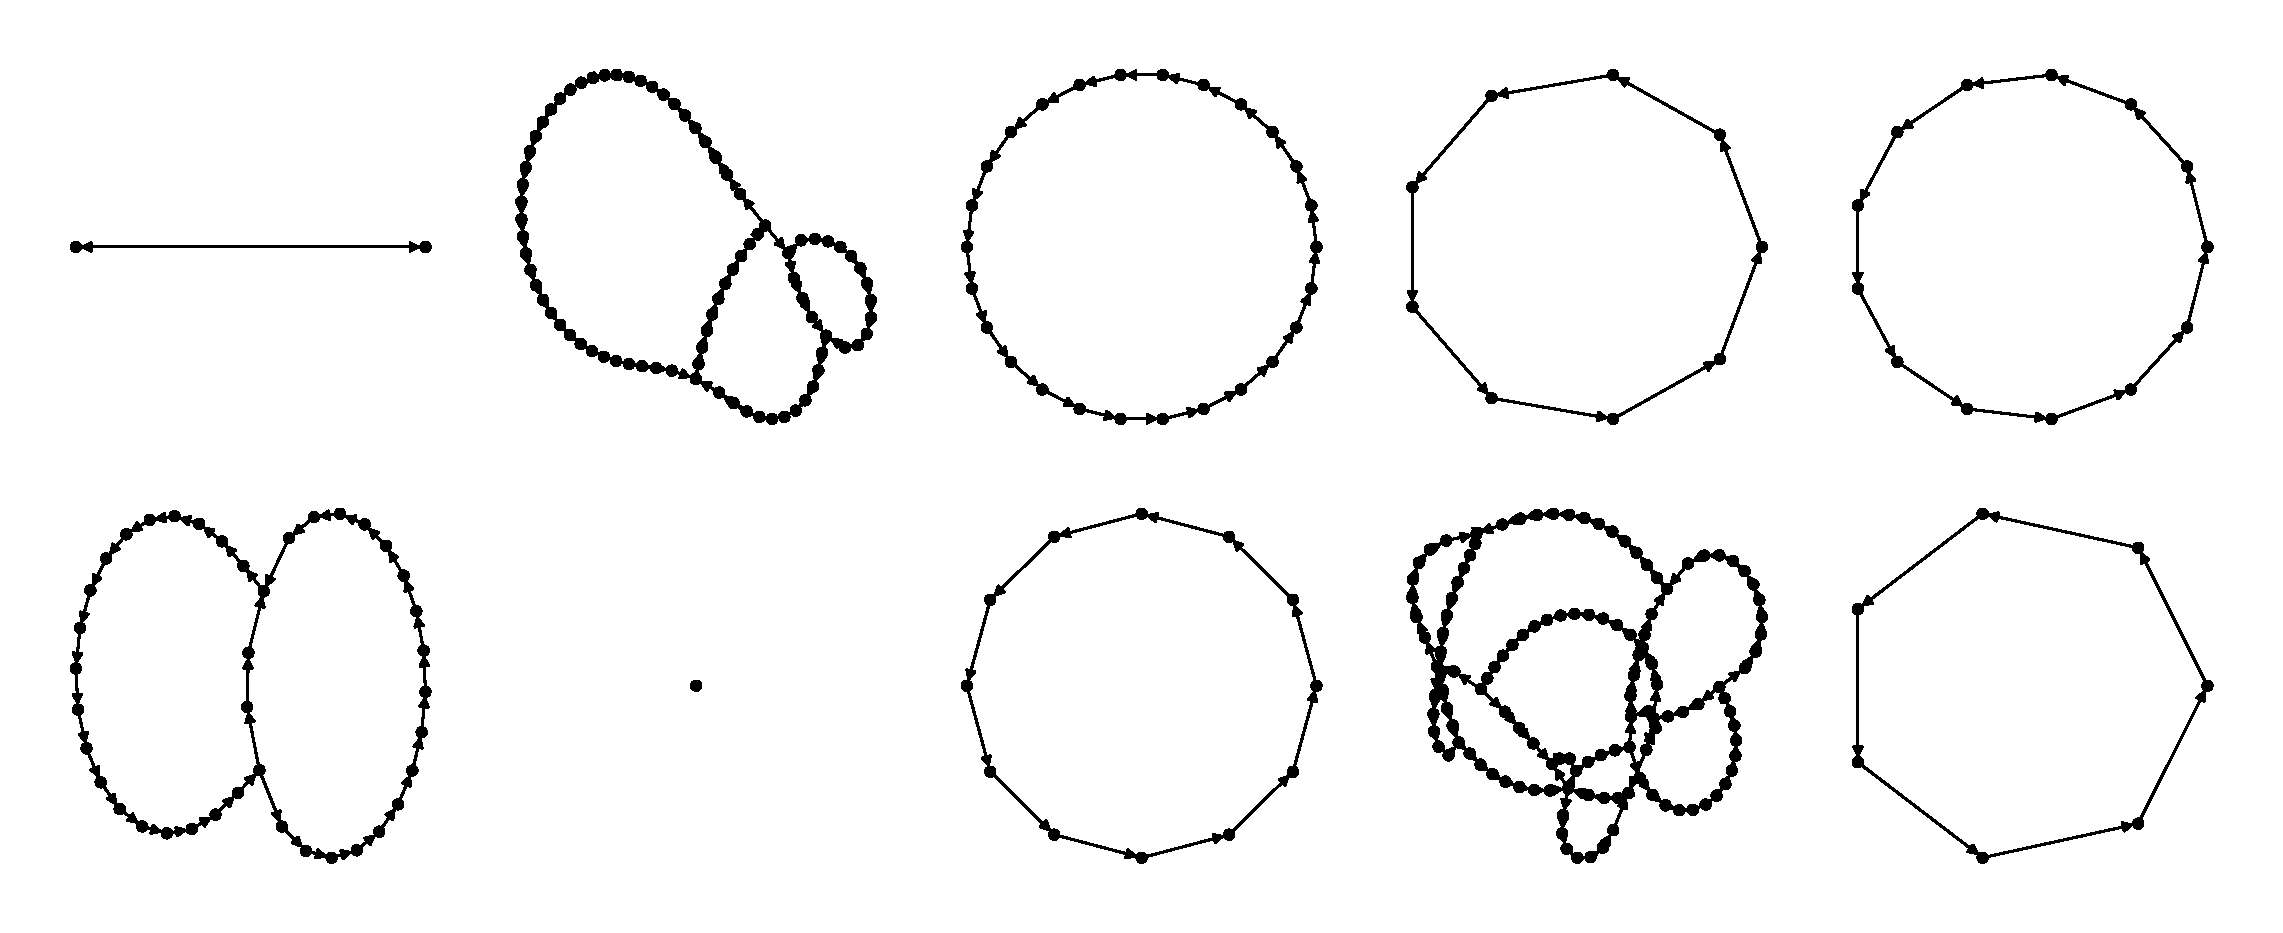
\includegraphics[width=\textwidth]{Content/Pictures/Fig3.eps}
    
    \caption{The largest SCC from samples of a directed configuration model with independent $\text{Poisson(1)}$ in- and out-degrees}
    \label{fig:largest-sccs}
\end{figure}

Figure \ref{fig:largest-sccs} shows the largest SCC from samples of a directed configuration model. As can be seen, while the lengths of paths in the SCC are long, the actual structure of the SCC is often quite simple. Previous work by \citet{goldschmidtScalingLimitCritical2021}, studying the directed Erd\H{o}s-R\'{e}nyi graph, formalised this using \emph{metric directed multigraphs} (MDMs), and we follow the same approach. These are simply weighted directed multigraphs, but in our context it is more appropriate to think of the weights as lengths, which motivates the change in naming. Formally, a \emph{directed multigraph} is a triple $(V, E, r)$ where
\begin{enumerate}
    \item $V$ is a set of \emph{vertices},
    \item $E$ is a set of \emph{edges}, and
    \item $r: E \to V \times V$ is a function mapping each edge to its \emph{head} and \emph{tail}; associated with $r$ are two functions $r_1: E \to V$ and $r_2: E \to V$ such that
\begin{equation*}
    r(e) = (r_1(e), r_2(e))
\end{equation*}
for all $e \in E$. $r_1(e)$ is the tail of the edge $e$ and $r_2(e)$ is the head of the edge $e$.
\end{enumerate}
 Then a \emph{metric directed multigraph (MDM)} is a tuple $M = (V, E, r, l)$ where $(V, E, r)$ is a directed multigraph and $l:E \to [0, \infty)$. Let $\zeroloop$ denote the MDM consisting of a single vertex with a self-loop of length 0.

An \emph{isomorphism} between two MDMs $M = (V, E, r, l)$ and $M' = (V', E', r', l')$ is a pair of functions $(i_V, i_E)$ where $i_V: V \to V'$ and $i_E: E \to E'$ are bijections satisfying the relation
\begin{equation*}
    r'(i_E(e)) = (i_V(r_1(e)), i_V(r_2(e)))
\end{equation*}
for all $e \in E$. We say two MDMs are \emph{isomorphic} if there exists an isomorphism between them. In other words, isomorphic MDMs have the same graph structures for their underlying directed multigraphs up to a relabelling of the edges and vertices. Write $\iso(M, M')$ for the set of all isomorphisms between $M$ and $M'$.

We now define a distance $\distmdm$ between two MDMs $M$ and $M'$.  Any isomorphism between $M$ and $M'$ gives a correspondence between the edges of $M$ and the edges of $M'$. We can then take an $\ell_{\infty}$ distance between the lengths of the edges and finally take the isomorphism which minimizes this distance. If $M$ and $M'$ are not isomorphic, we set the distance to be infinite. Formally,
\begin{equation*}
    \distmdm(M, M') = \begin{cases}
        \inf_{(i_V, i_E) \in \iso(M, M')} \sup_{e \in E} \abs{l(e) - l'(i_E(e))} & \text{if $M$ and $M'$ are isomorphic,} \\
        \infty & \text{otherwise.}
    \end{cases}
\end{equation*}
Consider an MDM $M$ and a vertex $w \in M$ with in-degree 1 and out-degree 1 which is not a self-loop. Let $u$ and $v$ be the unique in-neighbour and out-neighbour of $w$ respectively. The MDM obtained by \emph{smoothing} $w$ is obtained by deleting the edges $e_1$ and $e_2$ such that $r(e_1) = (u, w)$ and $r(e_2) = (w, v)$, then adding an edge $e$ such that $r(e) = (u, v)$ and assigning it length $l(e) = l(e_1) + l(e_2)$. This is illustrated in Figure \ref{fig:smoothing}. 
\begin{figure}[htbp]
    \centering
    \begin{subfigure}[htbp]{0.45\textwidth}
        \centering
        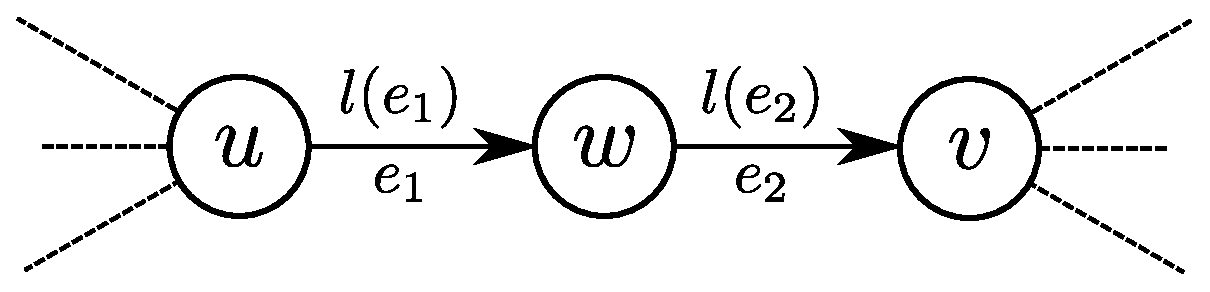
\includegraphics[width=0.95\textwidth]{Content/Pictures/Fig4a.eps}
        \caption{The graph before smoothing $w$}
    \end{subfigure}
    \hfill
    \begin{subfigure}[htbp]{0.45\textwidth}
        \centering
        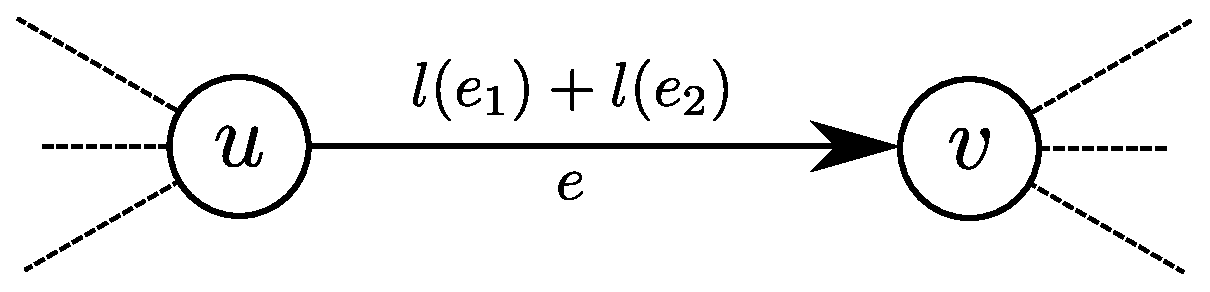
\includegraphics[width=0.95\textwidth]{Content/Pictures/Fig4b.eps}
        \caption{The graph after smoothing $w$}
    \end{subfigure}
    \caption{Smoothing a vertex $w$}
    \label{fig:smoothing}
\end{figure}

Then the kernel of a digraph $\vec{G}$ is obtained by doing the following:
\begin{enumerate}
    \item Assign length $1$ to each edge.
    \item Iteratively smooth vertices with in-degree 1 and out-degree 1 that are not self-loops until there are none remaining.
    \item Replace all singletons by $\zeroloop$.
\end{enumerate}
An example is shown in Figure \ref{fig:kernel}. We expect the graph structure of kernels of SCCs in the critical window to remain finite, whereas the lengths assigned to edges will tend to infinity.
\begin{figure}[htbp]
    \centering
    \begin{subfigure}[htbp]{0.45\textwidth}
        \centering
        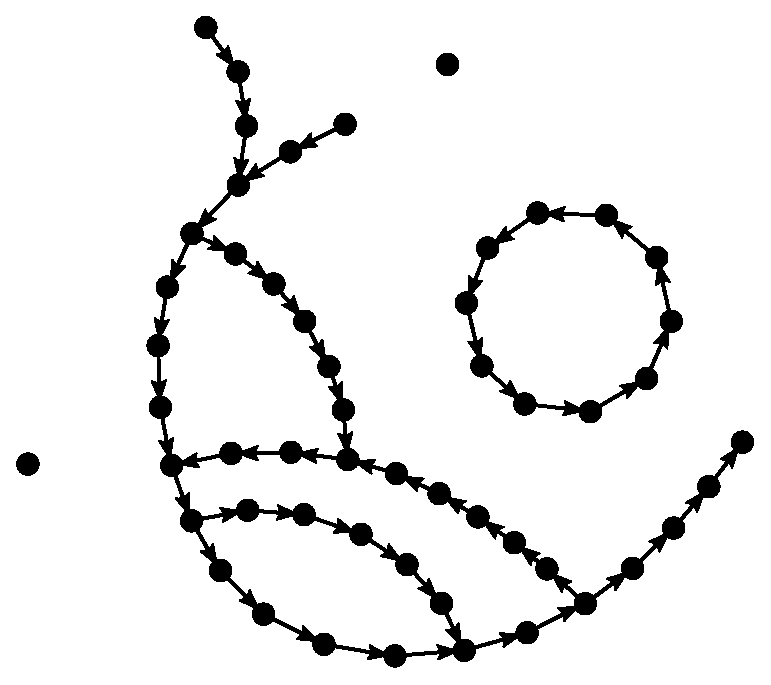
\includegraphics[width=0.90\textwidth]{Content/Pictures/Fig5a.eps}
        \caption{$\vec{G}$}
    \end{subfigure}
    \hfill
    \begin{subfigure}[htbp]{0.45\textwidth}
        \centering
        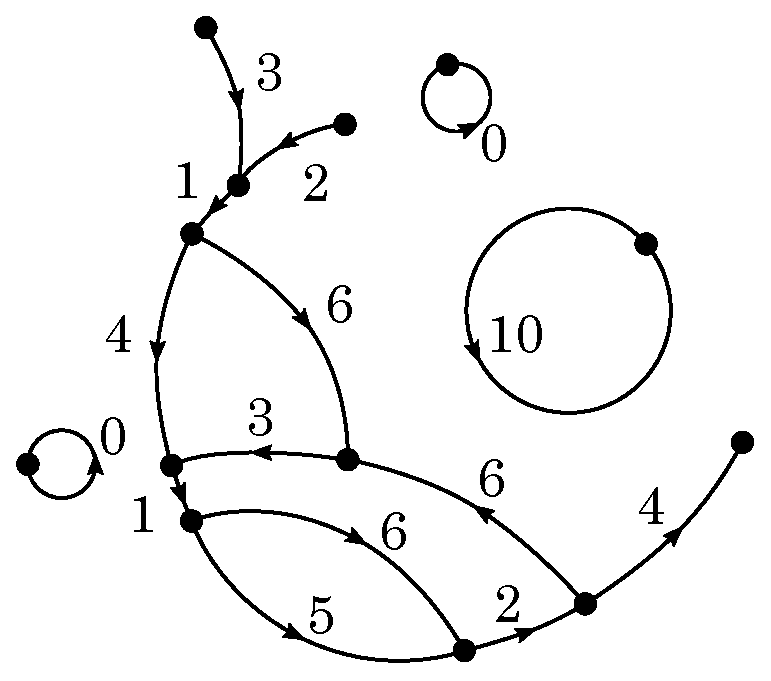
\includegraphics[width=0.90\textwidth]{Content/Pictures/Fig5b.eps}
        \caption{Kernel of $\vec{G}$}
    \end{subfigure}
    \caption{An example of a digraph $\vec{G}$ and its kernel. The numbers indicate the edge lengths.}
    \label{fig:kernel}
\end{figure}



\subsection{Our results}

For $M$ an MDM and $c\in (0,\infty)$, let $cM$ be equal to $M$ with all lengths multiplied by $c$. Let $C_i(n)$ for $i\geq 1$ be the kernels of the SCCs of $\vec{G}_n(\nu)$, listed in decreasing order of number of edges, breaking ties arbitrarily. Complete the list with an infinite repeat of $\zeroloop$. Then, our main theorem is as follows.
\begin{theorem}\label{thm.main}
There exists a sequence $\cC=(\cC_i,i\in \N)$ of random strongly connected MDMs such that 
$$\left(n^{-1/3}C_i(n),i\in \N\right)\todist\left(\cC_i,i\in \N\right)$$
as $n\to \infty$, with respect to the product $d_{\vec{\cG}}$-topology. The law of $\cC=(\cC_i,i\in \N)$ depends only on the parameters $\mu$, $\sigma_+$, and $(\sigma_{-+}+\nu_-)/\mu$. Further, for each $i\geq 1$, $\cC_i$ is either $3$-regular or a loop.
\end{theorem}
We will describe the limit object and some of its further properties in Subsection \ref{subsec.limitobject}.

The law of the limit object places some particular cases of our model in the universality class of the directed Erd\H{o}s--Rényi model as studied by \citet{goldschmidtScalingLimitCritical2021}. This is the content of the following corollary. The \emph{directed Erd\H{o}s--Rényi model} on $n$ vertices with parameter $p$, denoted by $\vec{G}(n,p)$, is a random digraph with vertex set $[n]$ in which each of the $n(n-1)$ possible directed edges is included with probability $p$ independently. The cases $p=(1+\lambda n^{-1/3})/n$ for $\lambda\in\R$ are referred to as \emph{the critical window}, and the case $p=1/n$ is called \emph{criticality}.

Note however that their result holds in a stronger topology: they use an $\ell_1$-like topology on the space of sequences of MDMs, whereas we show our result in the product topology. Due to this, it is important in their paper to consider singletons as loops of length zero. For any fixed $k$, the $k$th largest SCC will not be a singleton with high probability as $n \to \infty$. Therefore, no component of our limiting object will be a singleton and thus they need to pad their SCCs by $\zeroloop$ and consider the kernel of singletons to be $\zeroloop$, to prevent the $\ell_1$-distance, as defined by $d_{\vec{G}}$, between $\left(n^{-1/3}C_i(n),i\in \N\right)$ and $\left(\cC_i,i\in \N\right)$ being infinite. We follow the same convention.

\begin{theorem}\label{thm.erdosrenyi}
Consider $\vec{G}_n(\nu)$, with $\nu$ such that $$\mu=\sigma_+=\sigma_{-+}+\nu_-=1.$$ 
Let $(C^\nu_i(n), i\geq 1)$ be the kernels of the SCCs of $\vec{G}_n(\nu)$. Furthermore, let $(C^{ER}_i(n), i\geq 1)$ be the kernels of the SCCs of $\vec{G}(n,1/n)$. Then, $\left(n^{-1/3}C^\nu_i(n),i\in \N\right)$ and 
$\left(n^{-1/3}C^{ER}_i(n),i\in \N\right)$ have the same limit in distribution in the product-$d_{\vec{\cG}}$-topology as $n\to \infty$. 
\end{theorem}
Note that the condition in \Cref{thm.erdosrenyi} is satisfied by $\nu(k^-,k^+)=\nu_1(k^-)\nu_2(k^+)$, with $\nu_1$ and $\nu_2$ the law of a $\operatorname{Poisson}(1)$ random variable.

Moreover, Theorem \ref{thm.main} has the following trivial corollaries, which were previously unknown. 
\begin{corollary}\label{cor.componentsizes}
Let $E^i_n$ and $V^i_n$ be the number of edges and vertices in $C_i(n)$ respectively, both appended with infinite repeats of $0$. Then there exists a random sequence $(E_i,i\in \N)\in \R_+^\infty$, such that
$$\left(n^{-1/3}E^n_i,n^{-1/3}V^n_i, i\in \N\right)\todist\left(E_i,E_i,i\in \N\right)$$
as $n\to \infty$ in the product topology on $(\R^2)^{\N}$. 
\end{corollary}
In particular, note that, in the above corollary, the number of vertices and number of edges have the exact same scaling limit.
\begin{corollary}\label{cor.diameter}
For $v,w\in \vec{G}_n(\nu)$ such that $v\to w$, let $d(v,w)$ denote the length of the shortest directed path from $v$ to $w$, and let $$\operatorname{Diam}\left(\vec{G}_n(\nu)\right)=\max_{v,w\in V}\{d(v,w):v\to w\}$$ be the \emph{diameter} of $\vec{G}_n(\nu)$. Then, for any $\epsilon>0$, there is a $\delta>0$ such that $$\P\left( n^{-1/3}\operatorname{Diam}\left(\vec{G}_n(\nu)\right)>\delta\right)>1-\epsilon$$ for all $n$ large enough. Equivalently, $\operatorname{Diam}\left( \vec{G}_n(\nu) \right) = \Omega_p(n^{1/3})$.
\end{corollary}


\subsection{Previous work}\label{sec.previouswork}
The configuration model was introduced by \citet{bollobasProbabilisticProofAsymptotic1980} to sample a uniformly random undirected graph with a given degree sequence. (For a discussion of the configuration model and proofs of standard results, we refer the reader to \cite[Chapter 7]{hofstadRandomGraphsComplex2017}.)

Most results on the configuration model are proved for models with a deterministic degree sequence. The phase transition for the undirected setting was shown in \cite{molloyCriticalPointRandom1995, molloySizeGiantComponent1998, jansonNewApproachGiant2009}. The law of component sizes at criticality and in the critical window were obtained by \citet{riordanPhaseTransitionConfiguration2012} under the assumption that the degrees are bounded. Dhara, van der Hofstad, van Leeuwaarden and Sen showed convergence of the size and surplus edges in the critical window with a finite third moment \cite{dharaCriticalWindowConfiguration2017} and in the heavy-tailed regime \cite{dharaHeavytailedConfigurationModels2020}.  Bhamidi, Dhara, van der Hofstad and Sen obtained metric space convergence in the critical window in \cite{bhamidiUniversalityCriticalHeavytailed2020}, a result that the authors later improved to a stronger topology in \cite{bhamidiGlobalLowerMassbound2020}.

Configuration models with a random degree sequence are considered in \cite{josephComponentSizesCritical2014}, \cite{conchon--kerjanStableGraphMetric2021}, and \cite{Donderwinkel2021heightprocess}. \citet{josephComponentSizesCritical2014} showed convergence of the component sizes and surpluses of the large components under rescaling at criticality, both for degree distributions with finite third moments and for the heavy-tailed regime. \citet{conchon--kerjanStableGraphMetric2021} show Gromov-Hausdorff-Prokhorov convergence of the rescaled components ordered by decreasing size at criticality in these two regimes. The results in \cite{conchon--kerjanStableGraphMetric2021} in the heavy-tailed regime are extended to the critical window by the first author in \cite{Donderwinkel2021heightprocess}. Our techniques are closely related to the techniques introduced in \cite{conchon--kerjanStableGraphMetric2021}. 

Some results have been obtained for other directed graph models. \citet{caoConnectivityGeneralClass2019} consider a class of inhomogeneous directed random graphs. Their results include a phase transition for the existence of a giant SCC. This is a generalisation of work by Bloznelis, Götze and Jaworski in \cite{bloznelisBirthStronglyConnected2012}, in which a smaller class of inhomogeneous directed graphs is considered. Samorodnitsky, Resnick, Towsley, Davis, Willis and Wan \cite{samorodnitskyNonstandardRegularVariation2016} studied the tails of the degree distribution in the directed preferential attachment model. As previously mentioned, \citet{goldschmidtScalingLimitCritical2021} have studied the \emph{directed Erdős--Rényi model} in the \emph{critical window}, and were the first to obtain metric space convergence of the SCCs of a directed graph. Our methods build on their techniques. 

The directed configuration model was first considered by \citet{cooperSizeLargestStrongly2004}. They consider a deterministic degree sequence under a number of conditions. As discussed previously in \cref{subsec:model-description}, a phase transition for the SCCs occurs when a parameter $d$ is equal to 1. They show that for $d<1$, with high probability, all SCCs contain $O(\Delta\log(n))$ vertices, for $\Delta$ the maximal degree. On the other hand, for $d>1$, there is a unique SCC that contains a positive proportion of the vertices and edges. Their conditions are restrictive, and include finite second moments for both the in- and out-degree of a uniformly chosen vertex, and a bound of size $n^{1/12}/\log(n)$ on the largest degree. Their proofs are based on an algorithm to explore the directed graph. The condition on the largest degree was later relaxed to $O(n^{1/4})$ by \citet{grafStronglyConnectedComponents2016}. These results are in contrast with the critical case, with Corollary \ref{cor.componentsizes}, which says that in our set-up the number of vertices and edges in the largest strongly connected components are $\Theta(n^{1/3})$ in probability.

Recently, Cai and Perarnau have obtained a number of results on the directed configuration model with deterministic degrees. In \cite{caiDiameterDirectedConfiguration2020}, they show, under first and second moment conditions of the degree of a uniformly picked vertex, for $d\neq 1$ (i.e. not at criticality), that the diameter of the model on $n$ vertices, rescaled by $\log(n)$ converges to a constant that they identify. This is in contrast with Corollary \ref{cor.diameter}, which says that in our set-up the diameter is $\Omega(n^{1/3})$ in probability at criticality. Then, in \cite{caiGiantComponentDirected2021}, they show a law of large numbers for the number of vertices and edges in the largest SCC, under slightly stronger moment conditions, and again away from the critical point. In \cite{caiMinimumStationaryValues2021}, they study the behaviour of a random walk on a directed configuration model.
 
A necessary and sufficient condition for the existence of a giant weakly connected component for the directed configuration model with a deterministic degree sequence is discussed in the physics literature by \citet{kryvenEmergenceGiantWeak2016}. He also studies the distribution of the in- and out-components in \cite{kryvenFiniteConnectedComponents2017}.

The directed configuration model with random in- and out-degrees is also considered by \citet{chenDirectedRandomGraphs2013} although, importantly, they do not allow for the in- and out-degree of a vertex to be dependent. The authors consider a model in which the in- and out-degrees are two independent sequences of i.i.d.\ random variables drawn from different probability distributions. They propose an algorithm to sample degree sequences that correspond to a simple graph and show the limiting distribution of the degrees generated by this algorithm. 



\subsection{Proof outline}\label{sec:proofoutline}

\def \exploredvertices {\mathcal V}
\def \explorededges {\mathcal E}
\def \forest {F}
\def \edgestack {\mathcal Q}

Our techniques use height processes and \L ukasiewicz paths, which are standard objects used to encode trees and forests (see for instance \cite[Chapter 0]{AST_2002__281__R1_0}). We will introduce these here. Let $T=(V,E,\rho)$ be an ordered rooted finite tree with vertex set $V$, edge set $E$ and root vertex $\rho$; say $|V|=n$. Let $v_0,\dots,v_{n-1}$ denote the vertices of the tree visited in depth-first order, so that $v_0=\rho$. We can view $T$ as a metric space by regarding all edges as line segments of length $1$ that are connected via the vertices. The distance $d_T$ between points $a_1$ and $a_2$ on line segments $l_1$ and $l_2$ respectively is then defined as the length of the unique non-self-intersecting path between $a_1$ and $a_2$ that traverses the line segments of the tree. Denote $(T,d_T)$ by $\mathrm{T}$.\\
We will define the height process and \L ukasiewicz path of $\mathrm{T}$. Both of these functions uniquely characterize $\mathrm{T}$. The height process of $\mathrm{T}$, referred to as $h$, is defined as $$h(i)=d_T(v_i,v_0),$$ i.e.  for all $i$, $h(i)$ equals the distance from $v_i$ to the root.
Moreover, for all $i=1,\dots,n$, let $y_i$ be the number of children of $v_{i-1}$, and set $y_0=1$. Then, the \L ukasiewicz path of $\mathrm{T}$ is defined by $$s(i)=\sum\limits_{j\leq i} (y_j-1)$$ for $i=0,\dots,n$. Then, $s(i)$ is the total number of younger siblings of $v_i$ and its ancestors.
For a sequence of ordered rooted finite trees, we define its height process by concatenating the height processes of the trees in the sequence. The \L ukasiewicz path is defined similarly. 

We will study the law of the SCCs of a uniform directed graph with degree sequence $(\mathbf{D}_1,\dots,\mathbf{D}_n)$, conditional on $\sum_{i=1}^n D^-_i=\sum_{i=1}^n D^+_i$ by exploring the configuration model in a depth-first manner. This sampling naturally gives rise to a directed subforest of the resulting multigraph, which we call the \emph{out-forest}. The sampling procedure is  described in \cref{alg:edfs}, and is also illustrated in Figure \ref{fig.configuration model}. The definition of the out-forest is illustrated in Figure \ref{fig.configuration modeloutforest}.  

\begin{figure}
    \begin{subfigure}[htbp]{\textwidth}
        \centering
        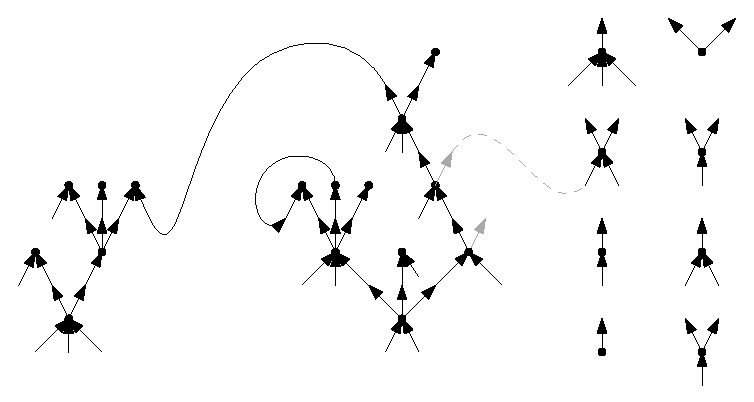
\includegraphics[scale=1]{Content/Pictures/Fig6a.eps}
        \caption{The gray arrows represent unpaired out-half-edges of vertices that have been discovered. One by one, in depth first order, these are paired to a uniform unpaired in-half-edge.}
        \label{fig.configuration model}
    \end{subfigure} \\

    \vspace{2em}

    \begin{subfigure}[htbp]{\textwidth}
        \centering
        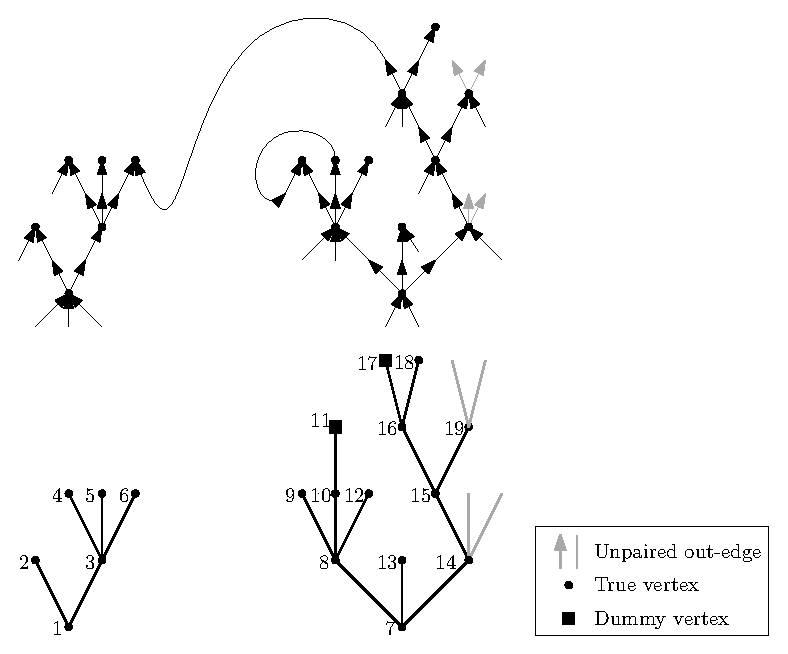
\includegraphics[scale=1]{Content/Pictures/Fig6b.eps}
        \caption{The out-forest is defined based on the exploration of the digraph. For each surplus edge, we add a dummy leaf. The labels of the vertices correspond to the time step in the exploration at which the vertex is added. The gray edges lead to vertices of which we do not know whether it is a dummy vertex, and if not, what its degree is. }
        \label{fig.configuration modeloutforest}
    \end{subfigure}

    \caption{Partial constructions of the configuration model and out-forest}
\end{figure}

% This procedure differs from the exploration used by \citet{goldschmidtScalingLimitCritical2021}.  The eDFS takes as input a directed multigraph and uses a stack (ordered list) of edges. When the stack is empty, we are at the start of a new out-component and pick a new vertex $w$ with probability proportional to its in-degree. Otherwise we remove the last edge $(v, w)$ from the stack. In both cases, if $w$ is not yet in the list of discovered vertices, we add the out-edges from this vertex to the \emph{end} of the stack of edges (this choice is what makes the exploration depth-first) and add $w$ to the list of discovered vertices $\exploredvertices$.  The order in which vertices are added to $\exploredvertices$ is referred to as their \emph{order of discovery}. Note that we will not discover any vertex with in-degree 0. From the perspective of finding the SCCs, this is not a problem since such vertices will form singleton SCC.

The sampling procedure uses a queue of unpaired out-edges (represented by the label of their corresponding vertex). When the queue is empty, we are at the start of a new out-component and pick a new vertex $w$ with probability proportional to its in-degree if there are vertices with positive in-degree remaining. Else, we pick a new vertex uniformly at random. If the queue is not empty, we pair the first out-edge in the queue to a uniform unpaired in-edge and call the corresponding vertex $w$. In both cases, if $w$ is not yet in the list of discovered vertices, we add the out-edges from this vertex to the \emph{front} of the queue of edges (this choice is what makes the exploration depth-first) and add $w$ to the list of discovered vertices. The order in which vertices are added to the list of discovered vertices is referred to as their \emph{order of discovery}. 

This procedure will discover vertices with in-degree 0 last. This is fine since such vertices form singleton SCCs, so we have discovered the non-trivial SCCs first.

\begin{algorithm}[htbp]
    \SetAlgoLined
    \KwData{A set of vertices $V=\{v_1,\dots, v_n\}$ with degree pairs $(d^-(v_1),d^+(v_1)),\dots, (d^-(v_n),d^+(v_n))$ satisfying $\sum d^-(v_i)=\sum d^+(v_i)$}
    $\exploredvertices \leftarrow$ an empty ordered list of vertices \tcp*[f]{the list of discovered vertices}\;
    $\edgestack \leftarrow$ an empty ordered list of vertices \tcp*[f]{the queue}\;
    $(d^-_{\mathrm{unpaired}}(v_1),\dots,d^-_{\mathrm{unpaired}}(v_n))\leftarrow (d^-(v_1),\dots,d^-(v_n))$  \tcp*[f]{the number of unpaired in-edges per vertex}\;
    $k \leftarrow 0$ \tcp*[f]{the index of the current step} \;
    $\hat{s}^- \leftarrow 0$ \tcp*[f]{the number of unpaired in-edges of discovered vertices}\;
    $\hat{s}^+ \leftarrow 1$ \tcp*[f]{the queue size minus the number of explored out-components} \;
    $\forest \leftarrow$ a directed forest with vertices $V$ and no edges
    \tcp*[f]{current out-forest}\;
     $M \leftarrow$ a directed multigraph with vertices $V$ and no edges
    \tcp*[f]{current di-multigraph}\;
    \While(){there exist undiscovered vertices OR $\edgestack$ is non-empty}{
        \eIf(\tcp*[f]{we start a new out-component}){$\edgestack$ is empty}{
            \eIf(){there exist undiscovered vertices with positive in-degree}{
            $w\leftarrow$ a random vertex not in $\exploredvertices$ chosen with prob.\ proportional to $d^-(w)$ \;}
            {$w\leftarrow$ a uniformly random vertex not in $\exploredvertices$}
            $\hat{s}^+\leftarrow \hat{s}^+-1$\tcp*[f]{we have explored a component}\;}{
            $v \leftarrow$ first entry in $\edgestack$ \tcp*[f]{we will pair an unpaired out-edge of $v$}\;
            remove first entry from $\edgestack$ \;
            $\hat{s}^+\leftarrow \hat{s}^+-1$\tcp*[f]{the queue size decreases by $1$}\;
            $w \leftarrow$ a random vertex chosen with prob.\ proportional to $d^-_{\mathrm{unpaired}}(w)$ \;
            add $(v,w)$ to $M$\tcp*[f]{we pair the out-edge of $v$ with a uniform unpaired in-edge}\;
            $d^-_{\mathrm{unpaired}}(w)\leftarrow d^-_{\mathrm{unpaired}}(w)-1$\;
            $\hat{s}^-\leftarrow \hat{s}^--1$\tcp*[f]{we have paired an in-edge}\;
            \eIf(\tcp*[f]{we sampled a surplus edge}){$w\in \exploredvertices$}{
            add a dummy leaf to $F$ and an edge from $v$ to the leaf\;}{
            add $(v,w)$ to $F$\;
            }
        }
        \If(){$w\not\in \exploredvertices$}{
        append $w$ to the end of $\exploredvertices$ \tcp*[f]{vertex $w$ is now discovered}\;
        append $d^+(w)$ repeats of $w$ to the start of $\edgestack$\;
        $\hat{s}^+\leftarrow \hat{s}^++d^+(w)$\tcp*[f]{the queue size has increased}\;
        $\hat{s}^-\leftarrow \hat{s}^-+d^-(w)$\tcp*[f]{the number of unpaired in-edges of discovered vertices has increased}\;
        }
        $k\leftarrow k+1$\;
        $\hat{s}^+_k\leftarrow \hat{s}^+$\;
        $\hat{s}^-_k\leftarrow \hat{s}^-$ \;
        }
    
    
    \caption{The edge depth-first configuration model \label{alg:edfs}}
\end{algorithm}
% \begin{algorithm}[htbp]
%     \SetAlgoLined
%     \KwData{A set of vertices $\{v_1,\dots, v_n\}$ with degree pairs $(d^-(v_1),d^+(v_1)),\dots, (d^-(v_n),d^+(v_n))$ satisfying $\sum d^-(v_i)=\sum d^+(v_i)$}
%     $\exploredvertices \leftarrow$ an empty ordered list of vertices \tcp*[f]{the list of discovered vertices}\;
%     $\edgestack \leftarrow$ an empty ordered list of vertices \tcp*[f]{the queue}\;
%     $(d^-_{\mathrm{unpaired}}(v_1),\dots,d^-_{\mathrm{unpaired}}(v_n))\leftarrow (d^-(v_1),\dots,d^-(v_n))$  \tcp*[f]{\# unpaired in-edges per vertex}\;
%     $\forest \leftarrow$ an empty directed graph
%     \tcp*[f]{the current out-forest}\;
%      $G \leftarrow$ an empty directed graph
%     \tcp*[f]{the current directed-graph}\;
%     \While(){there exist unpaired out-half-edges of vertices with positive in-degree}{
%         \eIf(\tcp*[f]{we are starting a new out-component}){$\edgestack$ is empty}{
%             $w \leftarrow$ a random vertex not in $\exploredvertices$ chosen with prob.\ proportional to $d^-(w)$ \;
%         }(){
%             $v \leftarrow$ last entry in $\edgestack$ \;
%             remove last entry from $\edgestack$ \;
%             $w \leftarrow$ a random vertex chosen with prob.\ proportional to $d^-_{\mathrm{unpaired}}(w)$\;
%         }
%         \eIf(){$w \not \in \exploredvertices$}{
%             append $w$ to $\exploredvertices$ \; 
%             add the vertex $w$ to $\forest$ \;
%             add the vertex $w$ to $M$ \;
%             \If(){$\edgestack$ is non-empty}{
%                 add the edge $(v, w)$ to $\forest$\;
%                 add the edge $(v, w)$ to $M$\;
%             }
%             append $d^+(w)$ repeats of $w$ to the end of $\edgestack$ \;
%         }{
%             add a dummy leaf to $\forest$ and and edge from $v$ to the leaf \tcp*[f]{we have discovered a surplus edge and add a dummy leaf to the forest} \;
%             add the edge $(v, w)$ to $M$\;
%         }
%     }
%     \While(){there exist unpaired out-half-edges}{
%     \eIf(){$\cQ$ is empty}
%     {$w\leftarrow$ a uniformly random vertex not in $\mathcal{V}$\;
%     append $w$ to $\mathcal{V}$\;
%     add $w$ to $M$\;}
%     {$v \leftarrow$ last entry in $\edgestack$ \;
%             remove last entry from $\edgestack$ \;
%             $w \leftarrow$ a random vertex chosen with prob.\ proportional to $d^-_{\mathrm{unpaired}}(w)$\;
%             $d^-_{\mathrm{unpaired}}(w)\leftarrow d^-_{\mathrm{unpaired}}(w)-1$ \tcp*[f]{we have paired an in-edge of $w$}\;
%             add the edge $(v,w)$ to $M$\;
%     }
%     }
    
%     \caption{The eDFS procedure \label{alg:edfs}}
% \end{algorithm}
% \begin{algorithm}[htbp]
%     \SetAlgoLined
%     \KwData{A set of vertices with degree pairs $(d^-(v_1),d^+(v_1)),\dots, (d^-(v_n),d^+(v_n))$ satisfying $\sum d^-(v_i)=\sum d^+(v_i)$}
%     $\exploredvertices \leftarrow$ an empty ordered list of vertices \tcp*[f]{the list of discovered vertices}\;
%     $\edgestack \leftarrow$ an empty ordered list of out-half-edges \tcp*[f]{the stack of out-half-edges}\;
%     $(d^-_{\mathrm{unpaired}}(v_1),\dots,d^-_{\mathrm{unpaired}}(v_n))\leftarrow (d^-(v_1),\dots,d^-(v_n))$  \tcp*[f]{the number of unpaired in-edges per vertex}\;
%     $k \leftarrow 0$ \tcp*[f]{the index of the current step} \;
%     $\hat{s}^- \leftarrow 0$ \tcp*[f]{the number of seen but unpaired in-edges}\;
%     $\hat{s}^+ \leftarrow 0$ \tcp*[f]{the total stack size minus the number of explored out-components} \;
%     $\forest \leftarrow$ an empty directed graph
%     \tcp*[f]{the current out-forest}\;
%      $G \leftarrow$ an empty directed graph
%     \tcp*[f]{the current directed-graph}\;
%     \While(){there exist unpaired out-half-edges of vertices with positive in-degree}{
%         \eIf(\tcp*[f]{we are starting a new out-component}){$\edgestack$ is empty}{
%             $w \leftarrow$ a random vertex not in $\exploredvertices$ chosen with prob.\ proportional to $d^-(w)$ \;
%             $\hat{s}^+ \leftarrow \hat{s}^+ - 1$ \tcp*[f]{we have finished exploring another out-component} \;
%         }(){
%             $e^+ \leftarrow$ last out-edge in $\edgestack$ \;
%             remove $e^+$ from $\edgestack$ \;
%             $v \leftarrow$ tail of $e^+$\;
%             $w \leftarrow$ a random vertex chosen with prob.\ proportional to $d^-_{\mathrm{unpaired}}(w)$\;
%             $d^-_{\mathrm{unpaired}}(w)\leftarrow d^-_{\mathrm{unpaired}}(w)-1$ \tcp*[f]{we have paired an in-edge of $w$}\;
%             $\hat{s}^- \leftarrow \hat{s}^- - 1$ \tcp*[f]{we have paired an in-edge} \;
%             $\hat{s}^+ \leftarrow \hat{s}^+ - 1$ \tcp*[f]{we have removed and edge from the stack} \;
%         }
%         \eIf(){$w \not \in \exploredvertices$}{
%             append $w$ to $\exploredvertices$ \; 
%             add the vertex $w$ to $\forest$ \;
%             add the vertex $w$ to $M$ \;
%             \If(){$\edgestack$ is non-empty}{
%                 add the edge $(v, w)$ to $\forest$\;
%                 add the edge $(v, w)$ to $M$\;
%             }
%             append all out-half-edges of $w$ to the end of $\edgestack$ in a uniform random order \;
%             $\hat{s}^- \leftarrow \hat{s}^- + d^-(w)$ \tcp*[f]{we have discovered $d^-(w)$ new unpaired in-edges} \;
%             $\hat{s}^+ \leftarrow \hat{s}^+ + d^+(w)$ \tcp*[f]{we have added $d^+(w)$ new edges to the stack}\;
%         }{
%             add a dummy leaf to $\forest$ and and edge from $v$ to the leaf \tcp*[f]{we have discovered a surplus edge and add a dummy leaf to the forest} \;
%             add the edge $(v, w)$ to $M$\;
%         }
%         $k \leftarrow k + 1$ \;
%         $\hat{s}^-_k \leftarrow \hat{s}^-$ \;
%         $\hat{s}^+_k \leftarrow \hat{s}^+$ \;
%     }
%     \While(){there exist unpaired out-half-edges}{
%     \eIf(){$\cQ$ is empty}
%     {$w\leftarrow$ a uniformly random vertex not in $\mathcal{V}$\;
%     append $w$ to $\mathcal{V}$\;
%     add $w$ to $M$\;}
%     {$e^+ \leftarrow$ last out-edge in $\edgestack$ \;
%             remove $e^+$ from $\edgestack$ \;
%             $v \leftarrow$ tail of $e^+$\;
%             $w \leftarrow$ a random vertex chosen with prob.\ proportional to $d^-_{\mathrm{unpaired}}(w)$\;
%             $d^-_{\mathrm{unpaired}}(w)\leftarrow d^-_{\mathrm{unpaired}}(w)-1$ \tcp*[f]{we have paired an in-edge of $w$}\;
%             add the edge $(v,w)$ to $M$\;
%     }
%     }
    
%     \caption{The eDFS procedure \label{alg:edfs}}
% \end{algorithm}
% \begin{algorithm}[htbp]
%     \SetAlgoLined
%     \KwData{A directed multigraph}
%     $\exploredvertices \leftarrow$ an empty ordered list of vertices \tcp*[f]{the list of discovered vertices}\;
%     $\edgestack \leftarrow$ an empty ordered list of edges \tcp*[f]{the stack of edges}\;

%     $k \leftarrow 0$ \tcp*[f]{the index of the current step} \;
%     $\hat{s}^- \leftarrow 0$ \tcp*[f]{the number of seen but unpaired in-edges}\;
%     $\hat{s}^+ \leftarrow 0$ \tcp*[f]{the total stack size minus the number of explored out-components} \;
%     $\forest \leftarrow$ an empty directed graph \tcp*[f]{the current out-forest}\;
%     \While(){there exist undiscovered vertices of positive in-degree}{
%         \eIf(\tcp*[f]{we are starting a new out-component}){$\edgestack$ is empty}{
%             $w \leftarrow$ a random vertex not in $\exploredvertices$ chosen with prob.\ proportional to $d^-(w)$ \;
%             $\hat{s}^+ \leftarrow \hat{s}^+ - 1$ \tcp*[f]{we have finished exploring another out-component} \;
%         }(){
%             $e \leftarrow$ last edge in $\edgestack$ \;
%             remove $e$ from $\edgestack$ \;
%             $v \leftarrow$ tail of $e$\;
%             $w \leftarrow$ head of $e$ \;
%             $\hat{s}^- \leftarrow \hat{s}^- - 1$ \tcp*[f]{we have paired an in-edge} \;
%             $\hat{s}^+ \leftarrow \hat{s}^+ - 1$ \tcp*[f]{we have removed and edge from the stack} \;
%         }
%         \eIf(){$w \not \in \exploredvertices$}{
%             append $w$ to $\exploredvertices$ \; 
%             add the vertex $w$ to $\forest$ \;
%             \If(){$\edgestack$ is non-empty}{
%                 add the edge $(v, w)$ to $\forest$\;
%             }
%             append all out-edges of $w$ to the end of $\edgestack$ in a uniform random order \;
%             $\hat{s}^- \leftarrow \hat{s}^- + d^-(w)$ \tcp*[f]{we've discovered $d^-(w)$ new unpaired in-edges} \;
%             $\hat{s}^+ \leftarrow \hat{s}^+ + d^+(w)$ \tcp*[f]{we've added $d^+(w)$ new edges to the stack}\;
%         }{
%             add a dummy leaf to $\forest$ and and edge from $v$ to the leaf \tcp*[f]{we've discovered a surplus edge and add a dummy leaf to the forest} \;
%         }
%         $k \leftarrow k + 1$ \;
%         $\hat{s}^-_k \leftarrow \hat{s}^-$ \;
%         $\hat{s}^+_k \leftarrow \hat{s}^+$ \;
%         $\forest_k \leftarrow \forest$ \;
%     }
%     \caption{The eDFS procedure \label{alg:edfs}}
% \end{algorithm}

At each step we also track two natural numbers $\hat{s}^-(k)$ and $\hat{s}^+(k)$. The first one, $\hat{s}^-(k)$ keeps track of the number of unpaired in-edges of discovered vertices at time $k$. The second one, $\hat{s}^+(k)$ is akin to a \L{}ukasiewiscz path. At any given step it is equal to the size of the queue after subtracting the number of fully explored out-components.

We also construct a directed forest for which $\hat{s}^+(k)$ will be the true \L{}ukasiewicz path. At each step of the process we will examine a vertex $w$. If $w$ has not been discovered yet then either we are at the start of a new out-component, in which case we make $w$ the root of the next out-component, or we added an edge $(v, w)$ to the multigraph with $v$ already discovered, in which case we add the edge $(v, w)$ to the out-forest as well. If $w$ has already been explored we cannot add $(v, w)$ to the out-forest without creating cycles or connecting two different components. We instead add a \emph{dummy leaf} to the out-forest and an edge from $v$ to the dummy leaf.  We call any vertex that is not a dummy leaf a  \emph{true vertex}. This is illustrated in Figure \ref{fig.configuration modeloutforest}.


Consider an edge $(v,w)$ in the directed multigraph. If $(v, w)$ is not in the out-forest we refer to the edge as \emph{surplus}. Such an edge will instead correspond to an edge $(v, d)$ in the out-forest where $d$ is a dummy leaf. 

An important motivation for studying the out-forest is the fact that the vertex set of any SCC is contained in one of the components of the out-forest. This is a straightforward property which we will prove below as part of \cref{lem:whatispartofscc}. Moreover, we defined the out-forest in such a way that every time step in the exploration corresponds to one vertex in the out-forest.

Our technique relies on dismissing surplus edges that cannot be part of a strongly connected component (for example, surplus edges between two different out-components cannot form a directed cycle and are never part of a strongly connected component). We define a necessary condition for a surplus edge to be part of an SCC (see Definition \ref{def.candidate} and \cref{prop:edgesinSCCs}), and we call dummy leaves that correspond to surplus edges with this property \emph{candidates}. Then, we define a procedure to sample only the out-forest and the edges corresponding to candidates, which allows us to find the SCCs.

We note the following key facts. Firstly, the order in which the true vertices are discovered does not depend on the positions of the dummy leaves. Secondly, the positions of the dummy leaves do not depend on the position of the heads of the surplus edges. Finally, whether a dummy leaf is a candidate does not depend on the position of the heads of the surplus edges. This allows us to define the following step-by-step sampling procedure. 
\begin{enumerate}
    \item We sample the order of discovery of the true vertices.
    \item We sample at which time steps we add a dummy leaf instead of a true vertex. 
    \item For each dummy leaf we sample whether it is a candidate.
    \item For each candidate we sample the position of the head of the corresponding surplus edge.
\end{enumerate}
For an exact description of the sampling procedure, see Subsection \ref{subsec.discrete}. The analogous sampling procedure for the limit object is described in Subsection \ref{subsubsec.samplecontinuousobject}. Then, our approach to show convergence is as follows.


\begin{enumerate}
    \item We find the limit under rescaling of the \L ukasiewicz path and height process of the out-forest up to time $m_n=\Theta(n^{2/3})$ conditional on the event $\left\{\sum_{i=1}^n D^-_i=\sum_{i=1}^n D^+_i\right\}$. This is the content of  \cref{prop:convoutforest}. Note that we condition on an asymptotically singular event, which causes significant difficulties.   Our method relies on a measure change between the sequence of degrees in order of discovery under this conditioning and a sequence of i.i.d.\ random variables in $\N\times\N$. In Section \ref{sec:measure-change} , we show the convergence of the measure change under rescaling.
    \item We establish that the positions of the tails of the surplus edges corresponding to the candidates converge. This is the content of Proposition \ref{prop.convergenceancestraledges}, Lemma \ref{prop.extractexcursions}, and Proposition \ref{prop.convergencestartingpointscandidates}.
    \item We show that the positions of the heads of the surplus edges corresponding to the candidates converge, which is the content of Proposition \ref{prop.convergenceheadscandidates}. 
    \item We identify the tails and heads of the surplus edges corresponding to the candidates, and recover the SCCs from the resulting digraph via a cutting procedure. We use a result from \cite{goldschmidtScalingLimitCritical2021} to show that the cutting procedure converges. This summarised in Corollary \ref{prop:sccordereduptotimeT}.
    \item We show that conditioning on the resulting multigraph being simple does not affect the sampling procedure on the time scale $O(n^{2/3})$. This is the content of Proposition \ref{prop.anomalousedges}. 
    \item We prove that for any $\delta>0$, with high probability, all SCCs with more than $\delta n^{1/3}$ edges are contained in the exploration up to time $O(n^{2/3})$. Therefore, we can choose $m_n$ such that, with high probability, we do not miss any large SCCs by not considering the exploration beyond time $m_n$, which finishes the proof of the convergence in the product topology. This is the content of Lemma \ref{lemma.largesccfoundfirst}. 
\end{enumerate}



